\documentclass[conference]{IEEEtran}
\usepackage{cite}
\usepackage[pdftex]{graphicx}
\usepackage{amsmath}
\usepackage[utf8]{inputenc}
\usepackage{multicol,caption}


\newenvironment{Figure}
  {\par\medskip\noindent\minipage{\linewidth}}
  {\endminipage\par\medskip}

% neat horizontal line
\newcommand{\HRule}{\rule{\linewidth}{0.5mm}}

\begin{document}

\title{TNM034 - Facial Recognition}

\author{\IEEEauthorblockN{Carl Englund}
\IEEEauthorblockA{caren083}
\and
\IEEEauthorblockN{Erik Sandrén}
\IEEEauthorblockA{erila135}
\and
\IEEEauthorblockN{Klas Eskilson}
\IEEEauthorblockA{klaes950}}

\maketitle

\begin{abstract}
Face recognition is a very difficult subject to master. This report will describe an implementation which was developed during a few weeks. The results which was gathered and a discussion of what could have been improved is provided.

\end{abstract}

\section{Introduction}
The art of detecting faces and recognizing them is a part of our everyday life. Facial recognition is used as an authentication system for our phones and laptops. With the increasing personal information stored on these devices, the need for the security and reliance of the recognition has to be increased as well. We also expect the recognition to work with any conditions in regard of lighting conditions and orientation. Within the research area of image processing, these implication of these obstacles can be eliminated or their effect decreased.

This project applied some of these techniques in the implementation of a facial recognition system with mixed result in regards of false rejection rate (FRR) and false acceptance rate (FAR). FRR measures the rate of which a face in the database is not recognized while FAR measures the incorrect of the wrong person in the database or a person not in the database at all.



\section{The problem}
The aim of this project was to create a facial recognition system that would be able to recognize faces from a database of images. The images could have been modified and transformed in different ways to alter their appearances and compared with the database with successful results. Faces that didn’t exist in the database would also be tested against the system. If the system found a face, it would respond with the id of that person in the database. The system would also report if a face wasn’t recognized as being part of the database. 

Three image databases were given. One of the databases (DB1) was supposed to be used as the reference database – these were the images the system was supposed to be able to recognise. Another database contained images of persons not in the database (DB0). The third (DB2) contained images of persons in the reference database, but where certain parameters were changed; the light might be brighter or darker, the background could be cluttered, the person out of focus and the white balance could be different from the first database as well as the person’s facial expression. This database constitutes a great challenge, since these images are different from those in the first database. In order to allow these images to be recognised, the normalization process needs to be thorough.

\section{Methodology}
For correct recognition of a face the system had to do pre-processes of the
image as well as normalization of the face’s orientation and position. The
face was then analyzed with Eigenfaces to compare with the database. Some of
the steps described below used an adaptive thresholding during detection. The
decision to do this was based on the will to not dismiss images and faces in
the early pre-process steps but rather dismiss it during the comparison with
the Eigenfaces.

A brief overlook of the needed steps, which are also described below, for the detection can be seen in figure \ref{fig:overlook}.

\begin{figure}[htbp]
  \centering
  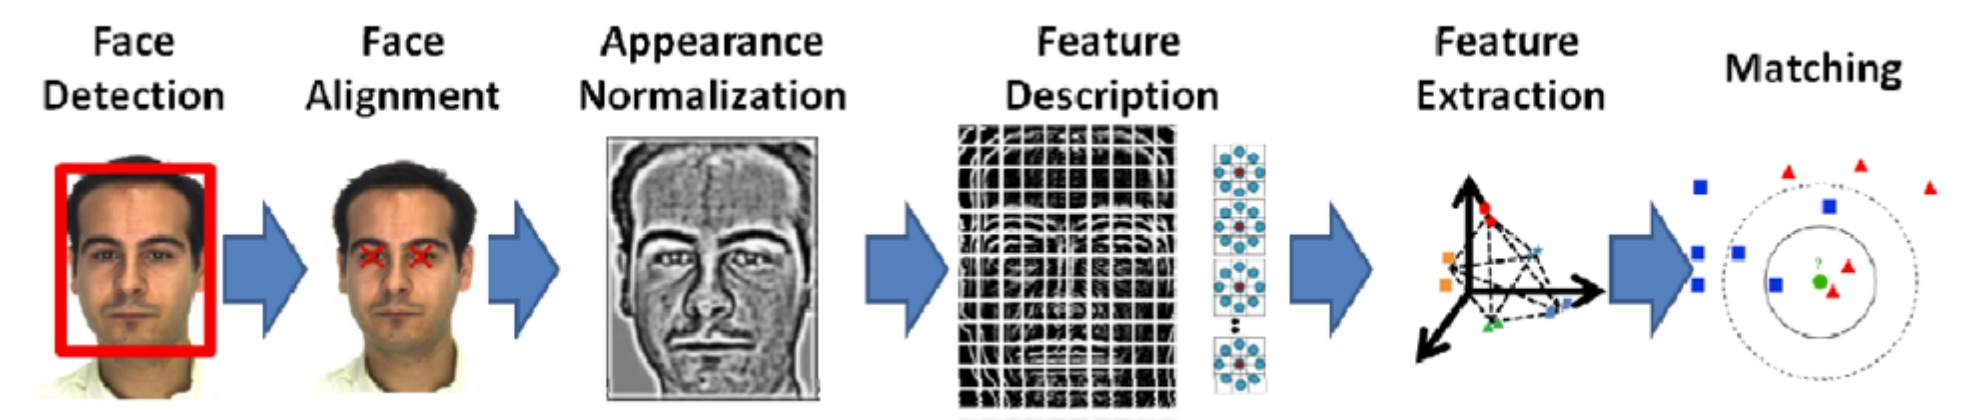
\includegraphics[width=\columnwidth]{images/process.jpg}
  \caption{Overlook of the whole face detection and recognition process.}
  \label{fig:overlook}
\end{figure}

\subsection{Lighting compensation}
Since the method of detecting a face in an image is based on color, the
potential difference in color temperature have to be eliminated. The method
used in this project was \emph{Gray world assumption}. The \emph{Gray world
assumption} method makes the assumption that the average value of the images
\emph{RGB} channels should be equal. The smallest average of the channels is
determined and then all the values in the image is scaled after this average
to eliminate any difference in white balance in images.

\subsection{Skin detection}
The first part of the recognition was to detect faces within an image. The
method used in this project was based on the implementation described by
AUTHOR2. The image’s color space was first converted from \emph{RGB} (Red,
Green, Blue) into \emph{YCbCr} (\emph{Y} being the brightness, \emph{Cb} the
blue chroma and \emph{Cr} the red chroma). The chroma channels were then
transformed into a value based on the brightness value of the pixels. This
transformation was done to be able to study the chroma values of each pixel in
a 2D space. The criteria for skin color was approximated to an ellipse in the
space of all chroma values that can be represented. The image was turned into
a binary image with only pixels within the ellipse set to white. This mask
would later be used as a mask to only show the skin areas, see figure \ref{fig:skinmask}. The last step of the skin detection was to dismiss all skin areas
except the biggest in the image and fills any holes in that area. The image
could then be cropped to this area to only contain the face part of the image.

\begin{figure}[htbp]
  \centering
  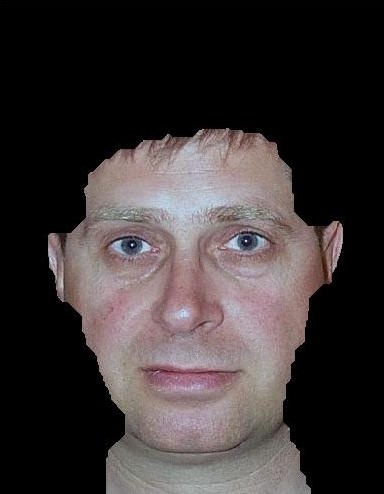
\includegraphics[width=0.6\columnwidth]{images/skinmask.jpg}
  \caption{The face mask applied to the original image.}
  \label{fig:skinmask}
\end{figure}

\subsection{Eye map}
When mapping eyes of a person a methodology presented in \cite{facedetection}
was used. The input image was converted into \emph{YCbCr} color space. This
was done since observations showed that high Cb values and low Cr values were
found around the eyes. Two different eye maps were calculated, one for the
chrominance part of the eye and one for the luminance part. To calculate an
eye map for the chrominance part equation \ref{eq:eyemapc} was used. For the
luminance part morphological operations was used to smooth out small and
irrelevant details. Equation \ref{eq:eyemapl} below was used to calculate the
luminance eye map.

\begin{equation}
  EyeMapC = \frac{1}{3}(C_b^2 + (\widetilde{C}_r)^2 + (C_b/C_r))
  \label{eq:eyemapc}
\end{equation}

\begin{equation}
  EyeMapL = \frac{Y(x, y)\oplus g_\sigma (x,y)}{Y(x, y)\ominus g_\sigma (x,y) + 1}
  \label{eq:eyemapl}
\end{equation}

To combine both eye maps elementwise multiplication was used. The combined eye
map is then dilated and masked in order to isolate the eyes. The result of the
eye detection can be seen in figure \ref{fig:eyemap}.

\begin{figure}[htbp]
  \centering
  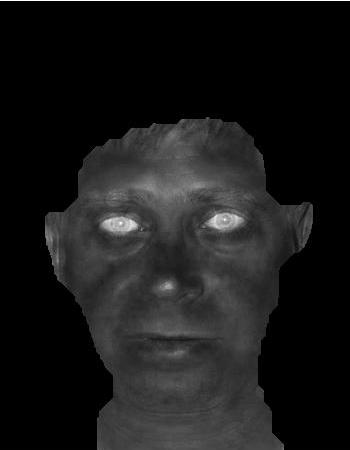
\includegraphics[width=0.6\columnwidth]{images/eye.jpg}
  \caption{The result of the eye map.}
  \label{fig:eyemap}
\end{figure}

\subsection{Mouth map}
The mouth map was calculated in a similar way to the eye map. By measuring the
different regions of the face the mouth can be detected based on the fact that
it usually has a strong red component in the facial region. The equation for
the map can be seen equations \ref{eq:mouthmap} and \ref{eq:moutheta}.
Similarly to the eye map the input image was converted into the YCbCr color
space and then processed.

\begin{equation}
  MouthMap = C_r^2 \cdot (C_r^2 - \eta \cdot C_r/C_b)^2
  \label{eq:mouthmap}
\end{equation}

\begin{equation}
  \eta = 0.95 \cdot \frac{\frac{1}{n}\sum_{(x,y)\in FG} C_r(x,y)^2}{\frac{1}{n}\sum_{(x,y)\in FG} C_r(x,y)/C_b(x,y)}
  \label{eq:moutheta}
\end{equation}

\subsection{Face alignment}
With the eye map and mouth map the important facial points could be found. The
maps were thresholded to create a binary mask. The maps were studied to find
the centroid of each white area in the mask. The different eye and mouth
candidates were then compared to each other to find the best face candidate.
The face was then warped to a normalized state with specific positions for the
eyes and mouth.

\subsection{LogAbout}
The purpose of the LogAbout method was to normalize the illumination of the
faces. This was to improve comparison in images where the the face had a wide
range of differently illuminated areas. The method was implemented using the
method suggested in \cite{logabout}. The input image was sent through a high
pass filter that can be seen in equation \ref{eq:filter}. When the filter had
been applied to the image it was transformed using a logarithmic function. The
equation used for the logarithmic function can be seen in equation
\ref{eq:logabout}.

\begin{equation}
  \begin{bmatrix}
    -1 & -1 & -1\\
    -1 & 9 & -1\\
    -1 & -1 & -1
  \end{bmatrix}
  \label{eq:filter}
\end{equation}

\begin{equation}
  g(x,y) = a + \frac{ln(f(x,y) + 1)}{b\cdot ln c}
  \label{eq:logabout}
\end{equation}

\subsection{Histogram equalization}
Similar to LogAbout, the purpose of histogram equalization was to normalize
the illumination of the faces. This method redistributes the image’s intensity
evenly throughout a larger spectrum in the histogram compared to before the
equalization. This resulted in an improved contrast in the image. \cite{histeq}
In theory, this could strengthen the distinguishing facial features of the images, but could also potentially increase the risk of failing to recognise
new features introduced to faces over time.

\subsection{Eigenfaces}
Storing and comparing a potentially large image database requires a lot of
memory, since each normalized image needs to be stored in a database and then
compared to the current image. If no action is taken to compensate for this, a
situation where the program’s memory requirements exceeds what is available is
likely to arise. To avoid this, and to lower the data size to a manageable
amount, a method called principal component analysis (PCA) was used. In
practice the number of dimensions in the high-dimensional dataset, that the
image database constitutes, is reduced.

This dimension reduction was performed by focusing on the difference between
the images. Correlated variables are not interesting when the aim is to
distinguish variance and make decisions upon differences. What was interesting
however was the uncorrelated variables. By calculating the mean image out of
all images in the database and subtracting this mean from a candidate image,
the unique features of the image were highlighted. This was used to calculate
the covariance matrices for the images, which in turn was used to calculate
eigenvalues and eigenvectors. These eigenvalues and eigenvectors were then
used to match candidate images with the images in the database. The resulting images can be seen in figure \ref{fig:eigen}.

\begin{figure}[htbp]
  \centering
  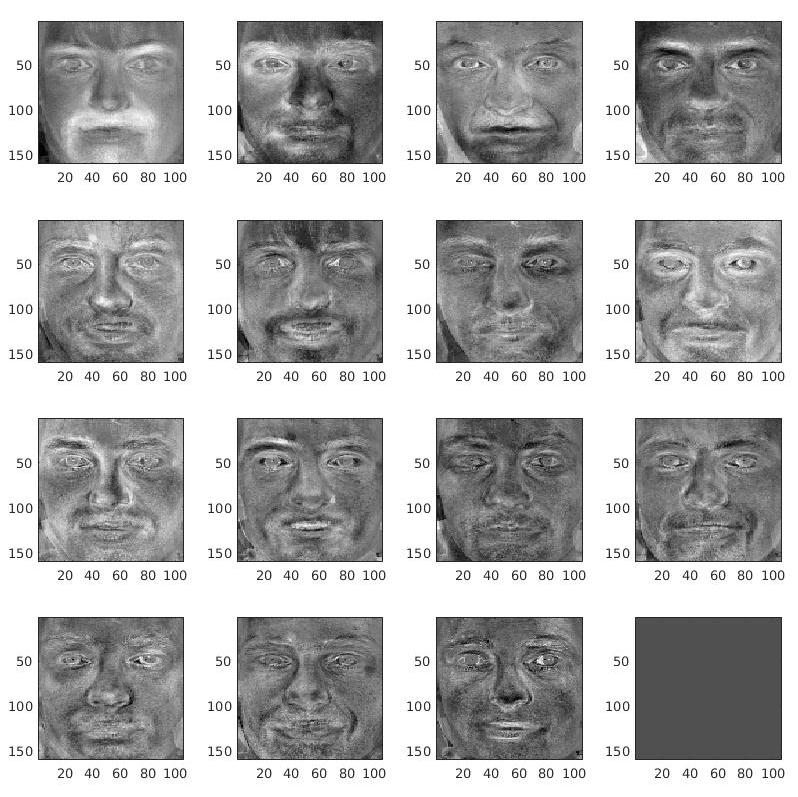
\includegraphics[width=\columnwidth]{images/eigen.jpg}
  \caption{Eigenfaces in the database.}
  \label{fig:eigen}
\end{figure}

\subsection{False negatives and false positives}
Naturally, the program errors in some cases. There are two cases that deserves
to be mentioned here; false negatives and false positives. False negatives are
when the system does not match a face it should know. This can occur because
the image is discarded in the thresholding of the summed error, when the
system isn’t satisfyingly certain of the result. False positives is when the
program simply guesses wrong, but with such a certainty that it passes the
thresholding that should stop it. The result amount of false negatives and
false positives can be studied with two rates, \emph{false rejection rate}
(FRR) and \emph{false acceptance rate} (FAR). FRR measures the rate in which a
face in the database is not recognized and rejected, while FAR measures the
rate of an unknown face mismatched with a face in the database.


\section{Implementations}
The program was implemented in Matlab. It consists of one main function that accepts an RGB image as its only input variable, and returns the number corresponding to the correct face in the image database, if found.

Initially, the images are color-corrected using the gray world-assumption method. The largest RGB value is detected and used to normalize every channel. The image’s color-space is then converted to YCbCr using Matlab’s built-in function. The chroma channels of the image are then transformed through an implementation of the methods and equations described above.

When the chroma channels have been transformed we go further on and retrieves the mask for the face as well as the mouth and eye map as described above.

After completing the steps for retrieving eyes and mouth we can form a triangle between our two eyes and our mouth. This helps later on to normalize all faces by performing a rotation of the faces. This is done by using Matlabs built in imwarp function. The pivot points for the imwarp are the left and right eye as well as the mouth.

In order to then further normalize the face we use histogram equalization to make sure all images have a somewhat even illumination. The result of this equalization can be seen below in figure N.

Figure N: Before and after histogram equalization.

When the normalization process has been performed it is all a matter of retrieving the eigenfaces from the images, a process that is described above. When the eigenface values for the candidate image is calculated, an error for each value in the reference database of eigenfaces is then calculated using the euclidian distance. The values in the Eigenface reference database are pre-calculated and stored in order to speed up the process, and to avoid re-calculating them for each candidate image. The ID of the image in the reference database that has the smallest euclidian error compared to the candidate image gets returned if the euclidian error passes a threshold of the maximum allowed error. This threshold value is found by taking the mean value of the error from all the false positives that the system returned during testing. This ID is what gets returned by the program.


\section{Result}
\subsection{Image enhancements}
All images tested in table 1 was retrieved from database one. Different combinations of luminance, rotation and scaling had been performed on the images according to the given boundaries in the task. In order to do this a testing program was set up that iterated over the different settings. All images were transformed with values where rotation started at -5 degrees, the tone value was decreased by -30\%, and the images were scaled down by 10\%. The program then iterated stepwise over these values until their positive counterpart was reached, obtaining each unique combination of distortions.

\begin{table}
    \caption{Images with different types of enhancements, total number of images is 432.}
    \begin{tabular}{|l|r|r|r|r|}
    \hline
    \multicolumn{1}{|l|}{\textbf{Enhancements}} & \multicolumn{1}{l|}{\textbf{Recognized}} & \multicolumn{1}{l|}{\textbf{FRR}} & \multicolumn{1}{l|}{\textbf{FAR}} & \multicolumn{1}{l|}{\begin{tabular}[c]{@{}l@{}} \textbf{ Face}\\ \textbf{not found}\end{tabular}}    \\ \hline
    None                    & 39.6\%      & 18.4\%  & 49.7\%    & 0.0\%             \\ \hline
    Gray world              & 44.9\%      & 24.0\%  & 58.2\%    & 0.0\%            \\ \hline
    Chroma transformation   & 50,0\%      & 13.9\%  & 61.1\%    & 0.0\%             \\ \hline
    Histogram equalization  & 53.1\%      & 51.2\%  & 40.6\%    & 0.0\%             \\ \hline
    GW + chroma             & 56.2\%      & 21.5\%  & 55.6\%    & 9.3\%             \\ \hline
    GW + hist.eq            & 51.6\%      & 29.2\%  & 50.2\%    & 0.0\%             \\ \hline
    Chroma + hist.eq        & 56.0\%      & 24.7\%  & 59.0\%    & 0.0\%             \\ \hline
    All enhancements        & 54.9\%      & 46.5\%  & 57.4\%    & 9.3\%             \\
    \hline
    \end{tabular}
    \label{tbl:enhancements}
\end{table}

As can be seen the different enhancement techniques that are applied to the images help to increase the correction rate a lot. There is however a problem with faces not being found when all enhancements are applied, as well as when Gray world + Chroma transformation was combined.

In Table 2 the different databases are tested with all enhancements active. The faces in DB0 was supposed to not be recognized but some of them are in the test. This could be fixed with a lower tolerance in the weight error but that would also result in a higher amount of FRR.

\begin{table}
    \caption{Tests on new images of faces in database(DB2) and face not in database(DB0).}
    \begin{tabular}{|l|r|r|r|r|r|}
    \hline
    \textbf{Databases} & \begin{tabular}[c]{@{}l@{}} \textbf{Number} \\ \textbf{of images}\end{tabular} & \textbf{Recognized} & \textbf{FRR} & \textbf{FAR} & \begin{tabular}[c]{@{}l@{}} \textbf {Face} \\ \textbf{not found} \end{tabular} \\ \hline
    DB0         & 4                 & -             & -         & 25.0\%    & 0.0\%  \\ \hline
    DB0\textsuperscript{1}        & 108               & -             & -         & 13.0\%    & 25.9\% \\ \hline
    DB1         & 16                & 100\%         & 0.0\%     & 0.0\%     & 0.0\%  \\ \hline
    DB1\textsuperscript{1,2}      & 432               & 54.9\%        & 46.5\%    & 57.4\%    & 9.3\%  \\ \hline
    DB2         & 38                & 31.6\%        & 13.3\%    & 75.0\%    & 10.5\%  \\ \hline
    DB21        & 1026              & 28.4\%        & 11.3\%    & 90.0\%    & 18.7\% \\
    \hline
    \end{tabular}
    \textsuperscript{1}:images are modified with rotation -5/+5 degrees, -10/+10\% scaling -30\%/+30 tone values \\
    \textsuperscript{2}:Details of the result available in table 3.
    \label{tbl:recognition-result}
\end{table}

\begin{table}
    \caption{The result of 432 images from DB1 with the distortions mentioned above, 27 images per face. No matches means that no face was found in the image.}
    \begin{tabular}{|l|r|r|r|r|}
    \hline
    \textbf{Image nr.}   & \textbf{Correct matches}   & \textbf{No matches}       & \textbf{FRR}    & \textbf{FAR}       \\ \hline
    1           & 6 (22.2\%)        & -                & 22.2\% & 40.7\%    \\ \hline
    2           & 4 (14.8\%)        & -                & 33.3\% & 51.9\%    \\ \hline
    3           & 5 (18.5\%)        & -                & 37.0\% & 22.2\%    \\ \hline
    4           & 3 (11.1\%)        & -                & 18.5\% & 70.4\%    \\ \hline
    5           & 10 (37.0\%)       & -                & 18.5\% & 37.0\%    \\ \hline
    6           & 10 (37.0\%)       & 7 (25.9\%)       & 33.3\% & 3.7\%     \\ \hline
    7           & 8 (29.6\%)        & 9 (33.3\%)       & 37.0\% & -         \\ \hline
    8           & 11 (40.7\%)       & -                & 59.3\% & -         \\ \hline
    9           & 1 (3.7\%)         & -                & 88.9\% & 7.4\%     \\ \hline
    10          & 6 (22.2\%)        & -                & 51.9\% & 25.9\%    \\ \hline
    11          & 7 (25.9\%)        & 3 (11.1\%)       & 37.0\% & 25.9\%    \\ \hline
    12          & 6 (22.2\%)        & -                & 44.4\% & 33.3\%    \\ \hline
    13          & 5 (18.5\%)        & -                & 40.7\% & 37.0\%    \\ \hline
    14          & 11 (40.7\%)       & -                & 22.2\% & 37.0\%    \\ \hline
    15          & 7 (25.9\%)        & -                & 18.5\% & 55.6\%    \\ \hline
    16          & 2 (7.4\%)         & -                & 44.4\% & 48.2\%    \\
    \hline
    \end{tabular}
    \label{tbl:breakdown}
\end{table}




\section{Discussion}
The result obtained in our face recognition system with DB1 is dependent on the images being taken in an environment with no distracting background. With this problem in mind there were problems getting any okay result at all on DB2, the database containing the challenging images of persons in the reference database. What happened was that the cluttered background contains skin-like parts that confuse the facial feature detection algorithm, and makes it think that there is skin where there is none. This leads to a situation where the skin detection, whose main purpose is to aid the eye and mouth detection, returns an unreasonably large mask. Within this large mask, there might be several eye and mouth candidates, which combined together creates faulty face candidates. An improvement of the implementation discussed in this paper could therefore be some better face detection method to easier mask out the areas with disturbance.

As can be seen in table 3, some images did not respond to the countermeasures taken against the distortion that the images were exposed to. Image number 9 only had one correct match out of 27, and in image number 7 there were 9 attempts where no face was found and the program canceled before any matching attempt were made. To understand what is going on in these particular cases, we take a look at the process of the face detection and normalization.

In figures \ref{fig:darkrotscal} to \ref{fig:mouth7}, the face detection process of image 7 is shown, where the image is darkened, rotated and scaled. As can be seen in figure \ref{fig:darkrotscal}, the face mask that is the result of the skin model function only returns a very small part of the whole face. This is the source of the issue – no face is detected since the eyes are excluded by the face mask. This is likely due to the lowered tone value of the image. 

\begin{Figure}
  % center it!
  \centering
    % adjust width as you like, include image from optional folder
    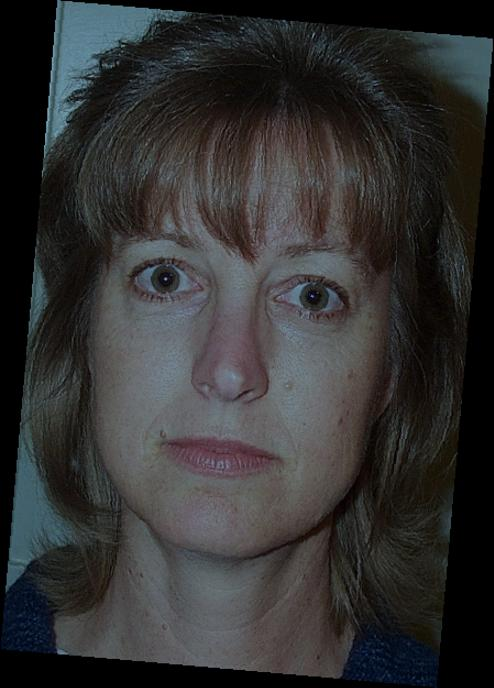
\includegraphics[width=0.5\columnwidth]{im7_img.jpg}
    % caption! change the label ref to what you want
    \captionof{figure}{\emph{Image 7 darkened, rotated and scaled}\label{fig:darkrotscal}}
\end{Figure}

\begin{Figure}
  % center it!
  \centering
    % adjust width as you like, include image from optional folder
    
\includegraphics[width=0.5\columnwidth]{im7_mask.jpg}
    % caption! change the label ref to what you want
    \captionof{figure}{\emph{Image 7 masked}\label{fig:mask7}}
\end{Figure}

\begin{Figure}
  % center it!
  \centering
    % adjust width as you like, include image from optional folder
    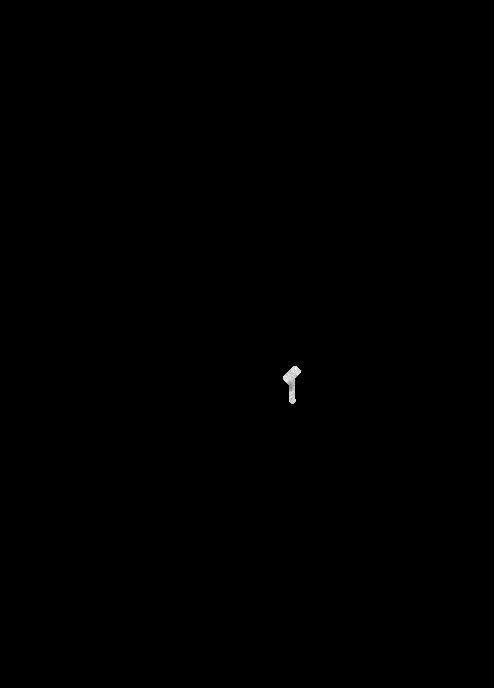
\includegraphics[width=0.5\columnwidth]{im7_eye.jpg}
    % caption! change the label ref to what you want
    \captionof{figure}{\emph{Eye map of image 7}\label{fig:eye7}}
\end{Figure}

\begin{Figure}
  % center it!
  \centering
    % adjust width as you like, include image from optional folder
    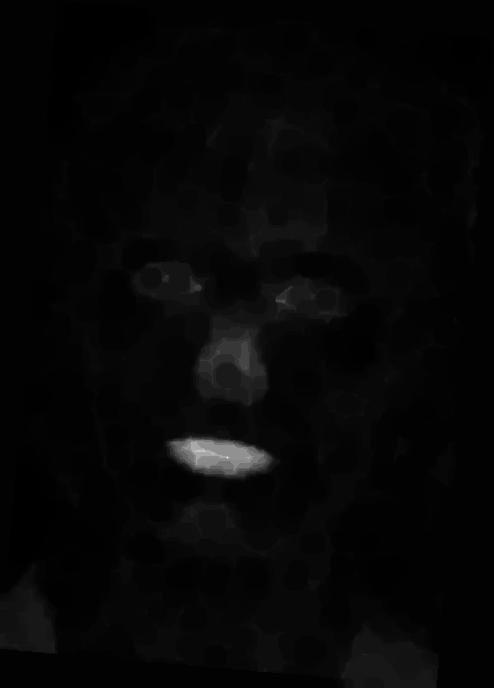
\includegraphics[width=0.5\columnwidth]{im7_mouth.jpg}
    % caption! change the label ref to what you want
    \captionof{figure}{\emph{Mouth map of image 7}\label{fig:mouth7}}
\end{Figure}


In figures \ref{fig:darkrotscal9} to \ref{fig:normalized9}, we see the completed detection and normalization of a rotated, lightened and scaled version of image 9. The normalization and facial detection works fine on this example, however it was registered as a false positive. The system guessed that this was a picture of another person. 


\begin{Figure}
  % center it!
  \centering
    % adjust width as you like, include image from optional folder
    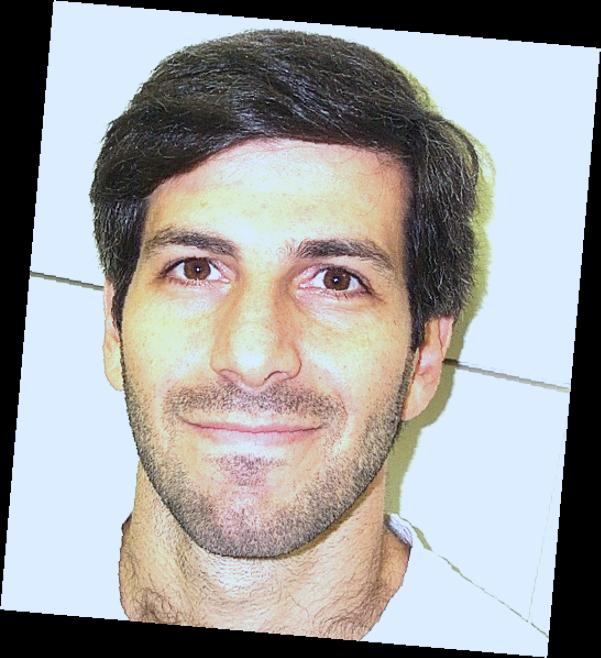
\includegraphics[width=0.5\columnwidth]{im9_img.jpg}
    % caption! change the label ref to what you want
    \captionof{figure}{\emph{Image 9 darkened, rotated and scaled}\label{fig:darkrotscal9}}
\end{Figure}

\begin{Figure}
  % center it!
  \centering
    % adjust width as you like, include image from optional folder
    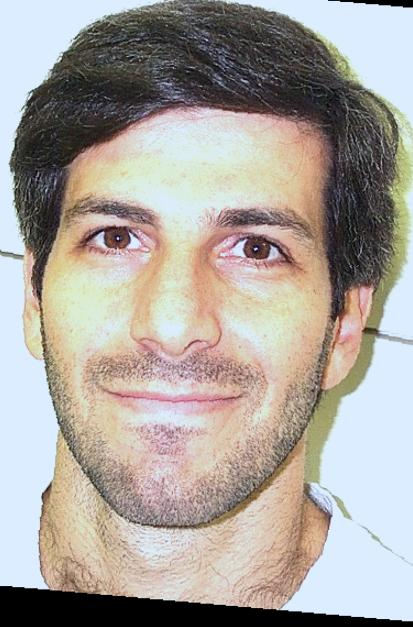
\includegraphics[width=0.5\columnwidth]{im9_cropped.jpg}
    % caption! change the label ref to what you want
    \captionof{figure}{\emph{Image 9 cropped}\label{fig:crop9}}
\end{Figure}

\begin{Figure}
  % center it!
  \centering
    % adjust width as you like, include image from optional folder
    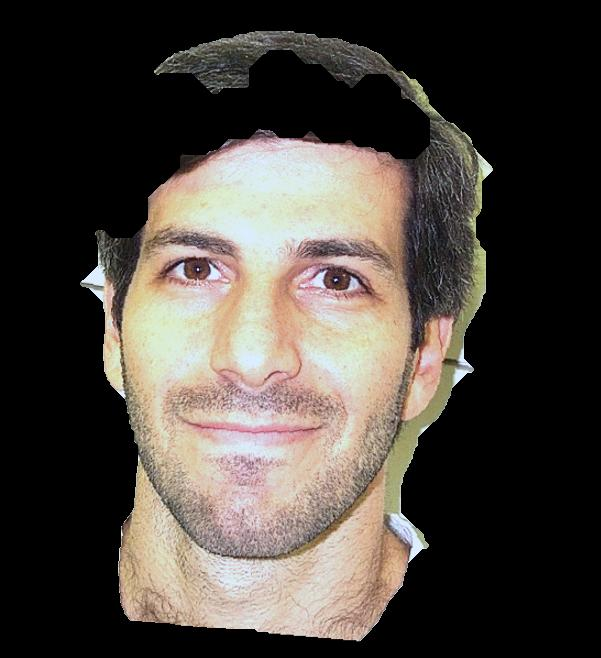
\includegraphics[width=0.5\columnwidth]{im9_mask.jpg}
    % caption! change the label ref to what you want
    \captionof{figure}{\emph{Image 9 masked}\label{fig:mask9}}
\end{Figure}

\begin{Figure}
  % center it!
  \centering
    % adjust width as you like, include image from optional folder
    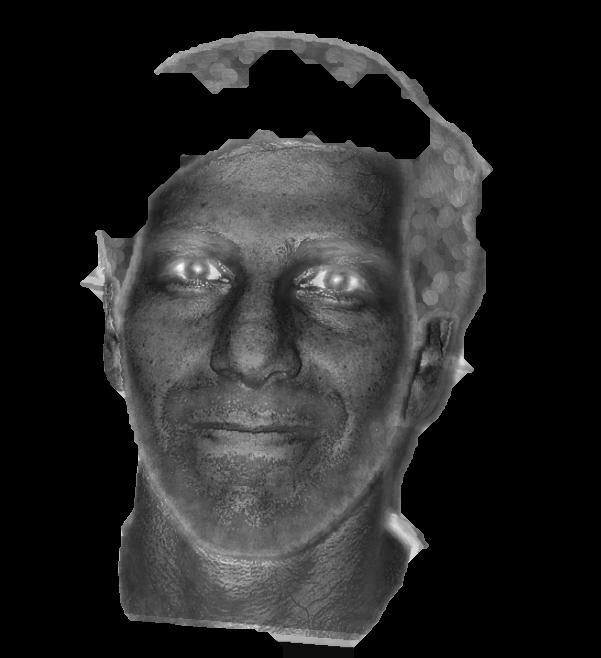
\includegraphics[width=0.5\columnwidth]{im9_eye.jpg}
    % caption! change the label ref to what you want
    \captionof{figure}{\emph{Eye map of image 9}\label{fig:eye9}}
\end{Figure}

\begin{Figure}
  % center it!
  \centering
    % adjust width as you like, include image from optional folder
    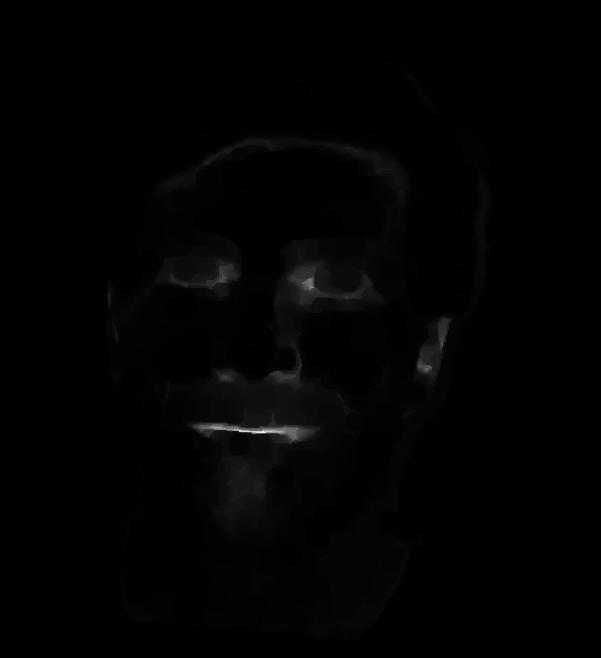
\includegraphics[width=0.5\columnwidth]{im9_mouth.jpg}
    % caption! change the label ref to what you want
    \captionof{figure}{\emph{Mouth map of image 9}\label{fig:mouth9}}
\end{Figure}

\begin{Figure}
  % center it!
  \centering
    % adjust width as you like, include image from optional folder
    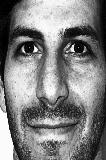
\includegraphics[width=0.5\columnwidth]{im9_normalized.jpg}
    % caption! change the label ref to what you want
    \captionof{figure}{\emph{Image 9 normalized}\label{fig:normalized9}}
\end{Figure}


\subsection{Fisherfaces}
One method that could have been used instead of Eigenfaces to increase the success of our recognition is Fisherfaces. FIsherfaces rely on linear discriminant analysis (LDA), a method that succeed Fisher's linear discriminant method (hence the name Fisherfaces) and that recognises patterns in a set of images. Similar to PCA, this method focus a lot on dimensionality reduction. This method would replace the Eigenfaces state, where the faces are recognised and not detected, of the system discussed here.

However, Fisherfaces is a method that greatly benefits from having several photos of the same class, in our case image of a face. Here, Fisherfaces focuses on maximizing the ratio of the between-class differences and the within-class differences (Eigenfaces vs. Fisherfaces: Recognition using class specific linear projection). Since we do know which class, again; face, each image belong to, we can use images from DB2 to create a better performing Fisherface database. This method can be considered more complex than Eigenfaces and relies on a solid and reliable facial detection system. Also, before this could be implemented, an improved face detection that works well on DB2 would have to be implemented.

According to Eigenfaces vs. Fisherfaces: Recognition using class specific linear projection, Eigenfaces has a higher error-rate when parameters such as lightning and expression vary. Therefore, the system is likely to benefit from an implementation of Fisherfaces. Other than the increased complexity, there isn’t really anything negative with Fisherfaces compared to Eigenfaces.


\subsection{LogAbout}
LogAbout was implemented and is available as an extra normalization feature in the program. However it was hard to find values that performed well for the given datasets. The problem that was  found was that it was hard to determine what values the constants a, b, and c should have in the equation. In the researched papers for the implementation of LogAbout there were no given constants since every dataset has its own values that fit for it.  Therefore attempts were made to determine the constants by trial and error. There were no good results that came out of this and it was settled that the LogAbout method were not to be used in our implementation since it only worsened the final result.


\section{Conclusion}
The face recognition process is something that a lot of research and time is put into. As stated in the beginning of this report a face that needs to be recognized could be rotated, have different illumination or a different scale than the reference image. Our implementation works for some of the images that have been changed, but it has been proven for us that it is very hard to implement a waterproof system.

Some improvements that could be implemented have been discussed. Mainly Fisherfaces could probably vastly improve the process, we do however not have that many training faces that seems to necessary for that implementation. Other methods that could improve our implementation also is for example the LogAbout method. This has been implemented but the results we achieved did not improve our implementation. There are reports that show the LogAbout method improving recognition rate however.


\begin{thebibliography}{1}

\bibitem{IEEEhowto:kopka}
H.~Kopka and P.~W. Daly, \emph{A Guide to \LaTeX}, 3rd~ed.\hskip 1em plus
  0.5em minus 0.4em\relax Harlow, England: Addison-Wesley, 1999.

\end{thebibliography}




% that's all folks
\end{document}

